\documentclass[12pt,fleqn]{article}\usepackage{../common}
\begin{document}
Paralel Lojistik Regresyon, Esle/Indirge

Lojistik regresyon kodunu esle-indirge (map-reduce) uzerinden paralelize
etmek icin literature [1-7] bakinca, genel yaklasimin makinalara bolunen
veri parcalari uzerinde ayri ayri graydan cikisinin (gradient ascent)
isletilmesi ve sonuc $\theta$'larin son bir makinada ortalamasinin alinmasi
oldugunu goruruz.

Daha onceki lojistik regresyon yazimizda iki farkli gradyan cikis
algoritmasi gormustuk. Bu algoritmalardan kullanacagimiz daha basit olani,
her dongude alpha'yi degistiren versiyon degil tek alpha kullanan, ve kod
icinde zar atan degil, veriyi sirayla isleyen. Bunun birkac sebebi var,
oncelikle altta gorecegimiz uzere veriyi Hadoop'a vermeden once kendimiz
karistiracagiz, yani kod icinde zar atmaya gerek kalmayacak. Ikincisi pek
cok makinada islem yapildigi icin tek bir sabit uzerinden azaltma yapmak
mumkun degil (fakat her isleyicinin -degismeyen- kendine has / ayri bir
sabiti olabilir, bu konuyu ileride isleyebiliriz), bu sebeple ve basitlik
amaciyla tek sabitli kod kullanildi. Ayrica artik dongu (iterasyon) yok,
yani veri bastan sona bir kez tarandi mi, o makinanin islemi bitecek. Fakat
buyuk veri ortaminda (ki zaten onun icin Hadoop kullaniyoruz herhalde)
elimizde o kadar cok veri olacak ki bu verinin tamamini isleyince zaten
100,200 kere donguyu isletmek ile ayni etkiyi almis oluyoruz.

Ornek veri olarak alttakini urettik,

\begin{minted}[fontsize=\footnotesize]{python}
from pandas import *
mean1 = [10,10]
mean2 = [20,20]
cov = [[5,0],[0,5]]             
d1 = DataFrame(np.random.multivariate_normal(mean1,cov,10000))
d2 = DataFrame(np.random.multivariate_normal(mean2,cov,10000))
d1['labels'] = 1
d2['labels'] = 0
data = DataFrame(np.vstack((d1,d2)))
data.to_csv("testSet.txt",sep='\t',index=None,header=None)
print data[:4]
\end{minted}

\begin{verbatim}
           0          1  2
0  10.287025  11.158653  1
1   7.390719  12.214295  1
2  11.720941   8.711403  1
3  11.543380  11.627805  1
\end{verbatim}

\begin{minted}[fontsize=\footnotesize]{python}
plt.plot(d1.ix[:,0],d1.ix[:,1],'b.')
plt.hold(True)
plt.plot(d2.ix[:,0],d2.ix[:,1],'r.') %
plt.hold(True)
plt.savefig('logreg1.png')
\end{minted}

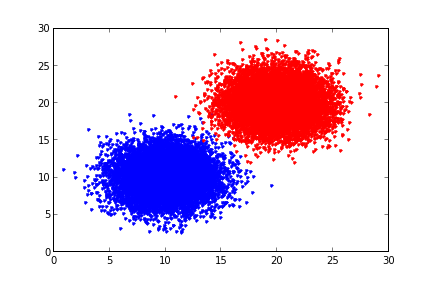
\includegraphics[height=6cm]{logreg1.png}

Altta veriyi isletmeden once kendimiz karistiriyoruz,

\begin{minted}[fontsize=\footnotesize]{python}
!sort --random-sort testSet.txt > /tmp/testSet1.txt
\end{minted}

\inputminted[fontsize=\footnotesize]{python}{logreg.py}

Ustte esleyici icinde tek bir tane anahtar uretiyoruz, tum makinalarda tum
esleyiciler ayni anahtari, bir kez uretiyor olacaklar. Bunun sebebi nedir?
Ne yapmaya calistigimizi hatirlayalim, tum makinalarda lojistik regresyon
isletiyoruz, gradyan cikisi yapiyoruz, ve sonucta o makinanin isi bitince
elimizde tek bir tane agirlik vektoru yani theta olacak. Ilgilendigimiz
sonuc bu, o yuzden cikti stdout'a tek bir satir yaziliyor. Peki niye ayni
anahtar? Cunku her makinadaki tum agirlik vektorlerinin "hep beraber" bir
noktada ortalamasinin alinmasini istiyoruz, bunu Hadoop'a yaptirmanin bir
yolu herkese ayni anahtari kullandirtmak, boylece bu anahtarlar tek bir
indirgeyiciye (ve makinaya) gidecek, ve orada ortalamalari alinacak. Tum
esleyicilerin sonucunun tek bir indirgeciye gitmesi performans problemi
cikartmaz mi? Cikmaz, cunku 1000 tane, 10000 tane esleyici paralel is
yapmis olabilir, ama isleri bitince elimizde 1000,10000 tane agirlik
vektoru olacak, ve bu zaten tek makinanin rahatlikla basa cikabilecegi bir
yuktur.

Bu yaklasim, esleyicinin her veri satiri basina bir ya da daha fazla
anahtar-deger satiri urettigi yaklasimdan (mesela klasik kelime sayma
problemi) biraz farkli, o sebeple bu farkliligi belirtmek istedik.

Bir puf nokta, her veri satiri icin isletilen map'e de aslinda anahtar
urettirmiyoruz, tum map cagrilari bittikten sonra son bir kez cagirilacak
map\_final'a bu isi yaptiriyoruz. Oraya gelinceye kadar (map icinde) degisen
theta'yi surekli hafizada tutmusuz, son noktaya gelince o sonucu ayni
anahtar ile esleyerek uretiyoruz ve is bitiyor.

Komut satirindan isletelim:

\begin{minted}[fontsize=\footnotesize]{python}
!python logreg.py /tmp/testSet1.txt 
\end{minted}

\begin{verbatim}
using configs in /home/burak/.mrjob.conf
creating tmp directory /tmp/logreg.burak.20131201.234703.391390
writing to /tmp/logreg.burak.20131201.234703.391390/step-0-mapper_part-00000
Counters from step 1:
  (no counters found)
writing to /tmp/logreg.burak.20131201.234703.391390/step-0-mapper-sorted
> sort /tmp/logreg.burak.20131201.234703.391390/step-0-mapper_part-00000
writing to /tmp/logreg.burak.20131201.234703.391390/step-0-reducer_part-00000
Counters from step 1:
  (no counters found)
Moving /tmp/logreg.burak.20131201.234703.391390/step-0-reducer_part-00000 -> /tmp/logreg.burak.20131201.234703.391390/output/part-00000
Streaming final output from /tmp/logreg.burak.20131201.234703.391390/output
"result"	"[[ 9.50705297]\n [-0.32580375]\n [-0.31237616]]"
removing tmp directory /tmp/logreg.burak.20131201.234703.391390
\end{verbatim}

\begin{minted}[fontsize=\footnotesize]{python}
def plot_theta(theta):
    x = np.array(arange(-10.0, 40.0, 0.1))
    y = np.array((-theta[0]-theta[1]*x)/theta[2])
    plot(x, y)
    hold(True)
    plot(d1.ix[:,0],d1.ix[:,1],'b.')
    hold(True)
    plot(d2.ix[:,0],d2.ix[:,1],'r.')
    hold(True)
    ylim(0,30)
    xlim(0,30)

theta = [9.50829527,-0.36317422,-0.34354905]
plot_theta(theta)
plt.savefig('logreg2.png')
\end{minted}

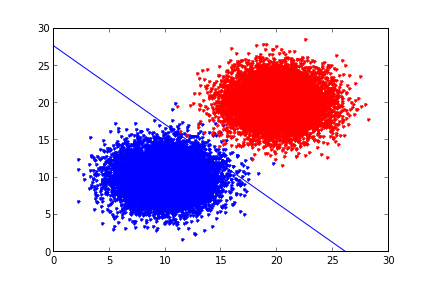
\includegraphics[height=5cm]{logreg2.png}

Kaynaklar

[1] http://alex.smola.org/teaching/berkeley2012/slides/4 Optimization.pdf

[2] http://cs.kangwon.ac.kr/~ysmoon/courses/2011 1/grad mining/slides/07-2.pdf

[3] http://www.slideshare.net/hadoop/modeling-with-hadoop-kdd2011

[4] http://www.xmarks.com/site/www.cs.stanford.edu/people/ang/papers/nips06-mapreducemulticore.pdf

[5] http://books.nips.cc/papersnips23/NIPS2010 1162.pdf

[6] http://simianer.de/P12-1002-slides.pdf

[7] http://www.holehouse.org/mlclass/17 Large Scale Machine Learning.html

[8] https://github.com/elsevierlabs/logistic-regression-sgd-mapreduce





\end{document}
